%!TEX root = Thesis_main.tex

\chapter{Control Theory}
\label{chapter3}
\section{Overview}
The interconnection between control theory and robotics has a history of over half a century during which control theory has developed solutions for problems in robotics field and problems in robotics have gained the new control theories. The goal of the early design of robotic systems was to develop mechanisms to be as stiff as possible modeled as single-input/single-output (SISO) linear systems with each joint controlled independently. Then Point-to-point control was used to perform simple tasks such as spot welding or pick and place operations. Encouraged by industry request, more complex tasks such as arc welding and spray painting have been enabled by Continuous-path tracking, but more advanced tasks like assembly were restricted by the limited or nonexistent sensing of the external environment. Higher speeds and higher payload-to-weight ratios required a better understanding of modeling of nonlinear dynamical systems. For this reason, new theoretical results in nonlinear, robust, and adaptive control enabled more advanced applications. Today, robot control systems are highly advanced with integrated sensing systems. Robot networks, surgical robots, mobile robots, underwater and flying robots, and others are starting to play important roles in society.\\
\textit{PID control} architecture is the most common form of feedback controllers. The first implementation of PID controllers dates back to early 20th century. Today more than 90\% of the control loops are PID type and are found in many areas. Nowadays it is often combined with other advanced control techniques where generally the main usage of PID based controllers is for low-level loops like motor controllers, integrated circuits etc. while advanced techniques are used for high-level control. In the case of mobile manipulators for pick and place operation the architecture of the online controller is generally hierarchic and the role of the PID regulator is to track desired high level control input.
The advantages of this basic control logic are the simplicity of implementation, lucid meaning, and the near-zero memory usage from the physical hardware. Because of that and the many tuning techniques developed in years, PID has been widely accepted in industry. Anyway, this basic feedback control law presents consistent limitations for advanced applications. 
\\
The \textit{inverse dynamics control} approach is directly related to the solution of the inverse dynamics problem of the system. Given the specified motion and the desired properties of the resulting system, the control inputs that ensure stability and realization of these control objectives are to be found. By appropriately inverting the dynamic model of the system to be controlled, a control law can be found. Generally this control law is chosen in order to cancel out the nonlinear part of the dynamics, to decouple the interactions between the regulated variables, and specify the behaviour of the convergence of the error. The inverse dynamics controller is able to enforce the execution of prescribed motion of the system and at the same time to control the interaction forces with the environment.
The usage of the inverse dynamics in robot control is widely diffused and allows to transform a MIMO nonlinear system into a simple decoupled linear system, nevertheless relies on a precise modeling of the dynamic system and a perfect knowledge of dynamical parameters. For those reasons classical inverse dynamics controllers are affected by changes in dynamical system properties more advanced techniques able to adapt to system modifications like \textit{Adaptive control} have been developed.  
\\
Adaptive controllers are different from other ordinary controllers because the control parameters are time-varying. Those parameters are adjusted by an online mechanism based on some signal of the closed-loop system. By means of this type of controller, it is possible to reach the control goal even if the plant is subjected to uncertainties or modifications. There are many ways in which this controller has been implemented, including adaptive computed-torque control, adaptive inertia-related control, adaptive control based on passivity, and adaptive control with desired compensation. 

\section{Optimal Control}
\begin{quote}
\textit{In place of determining the optimal sequence of decisions from the fixed state of the system, we wish
to determine the optimal decision to be made at any state of the system. Only if we know the latter, do
we understand the intrinsic structure of the solution.}
\emph{\begin{scriptsize}
Richard Bellman, Dynamic Programming,
1957. [Vinter, p. 435]
\end{scriptsize}}
\end{quote}
From a practical point of view, once the stability of a controller has been proved, nothing says that there is only one controller able to perform the control action. In other words since the stability proof does not determine a unique controller, generally it is possible to choose among different alternatives. It is pretty natural, in many contexts, that the choice of an optimal controller is preferred. The objective of optimal control theory, indeed, is to determine the control action that will cause a system to satisfy physical constraints and at the same time to minimize (or maximize) some performance criterion. Generally the definition of this criterion (i.e. cost function) is done according with the application of the controller. The design of an optimal controller generally relies on an exact model of the system. In fact, the presence of discrepancy between the model and the real system can lead to non-optimal solutions that can easily end in an unstable closed loop system. 
Let us consider a generic system described by nonlinear time-varying differential equation in $x\in \mathbb{R}^n$:
\begin{equation}
	\dot{x}(t)=f(x,t)+G(x,t)u
\end{equation}
where $u \in \mathbb{R}^m$ is the control input. Every optimal controller needs the definition of a cost function; for example, defining: 
\begin{equation}
	z=H(x,t)x+K(x,t)u
\end{equation}
such that: $H^T(x,t)K(x,t)=0$, $K^T(x,t)K(x,t)=R(x,t)>0$ and \\ $H^T(x,t)H(x,t)=Q(x,t)>0$, the quadratic cost function can be expressed as:
\begin{equation*}
	\frac{1}{2}z^Tz=\frac{1}{2}x^TQ(x,t)x+\frac{1}{2}u^TR(x,t)u
\end{equation*}
The optimal control law with a quadratic cost function can be derived from  the solution of HJB (Hamilton-Jacobi-Bellman) equation for a positive-definite function $V(x,t)$ as in \cite{kirk1970optimal}.
\begin{equation}
	\begin{split}
		0&=HJB(x,t,V)=V_t(x,t)+V_x(x,t)f(x,t) \\
		&-\frac{1}{2}		V_x(x,t)G(x,t)R^{-1 }		(x,t)G^T(x,t)V_x^T(x,t)+\frac{1}{2}Q(x,t)
\end{split}
\end{equation}

where $V_t=\frac{\partial V}{\partial t}$ and $V_x=\frac{\partial V}{\partial x^T}$. That defines the optimal controller such as:
\begin{equation}
	u=-R^{-1}(x,t)G^T(x,t)V_x^T(x,t) 
\end{equation}
A typical implementation of optimal control theory is made in practice by means of Model Predictive Control. 

\section{Model Predictive Control}
\label{section_MPC}

\epigraph{\textit{Discrete Dynamic Optimization Applied to On-line Optimal Control}}{\begin{scriptsize}
Rafal, Stevens, AiChE Journal, 1968
\end{scriptsize}}

The term Model Predictive Control (MPC from now on) designate a wide range of control strategies which use explicitly the model of the system to obtain the control action minimizing a specific cost function. The first development originated in the late seventies with IDCOM (Identification and Command) logic, using impulse response for the plant model and optimizing a quadratic objective function. This control, settled the basis of an architecture that has been developed considerably since then, expecially over the last two decades both within research community and industry.
Such a success is probably due to its generality, in fact MPC formulation can be considered as one of the most general ways to pose a process control problem. Its formulation can integrate optimal control, stochastic control, control of processes with dead time and multivariable control. In general nonlinear processes which are frequently found in industry, can be handled by MPC logics. Futhermore, unless stability and robustness proof is difficult to asses because of the finite horizon, it has been found to be quite robust in many applications. Anyway, although both in industry and in research is widely diffused, MPC has not reached yet the potential it suggests. One reason can be found in the fact that requires mathematical knowledge which is not usually available by control engineers in practice. This control architecture is generally an open framework that allows the development of many applications in use at the current time, not only in the industrial processes but also application to robotics, power plants, PVC plants, servos etc. 
\begin{table}
	\centering
	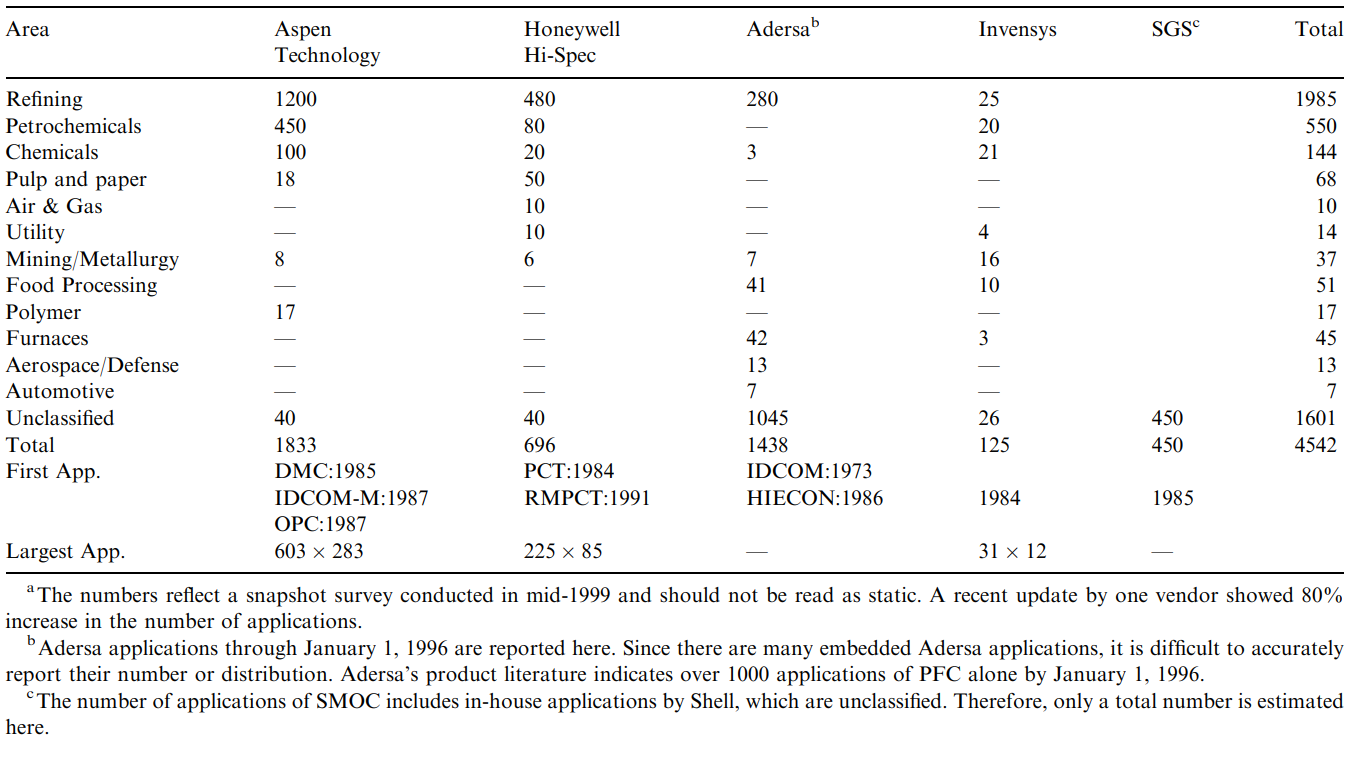
\includegraphics[scale=0.28]{mpc_usage_table}
	\caption{Summary of linear MPC applications by areas}
	\label{mpc_usage_table}
\end{table}
In \cite{qin2003survey} is presented an overview of industrial technologies where Model Predictive Control is used, both linear and nonlinear. Table \ref{mpc_usage_table} from that work shows the applications of MPC logic by area. Such a diffuse usage of this control logic collocate MPC as the second most used control methodology after PID. In the last decades MPC has been investigated in many fields such as Process control (linear or nonlinear MPC), Automotive (Explicit, Hybrid MPC), Aerospace(LTV MPC), ICT(distributed/decentralized MPC), Energy or Finance (stochastic MPC).Since MPC showed good performances in many of these applications as well as its ability to operate with few intervention for long periods of time, the interest in this control strategy has increasend in the last decades. This can be justified also by the increased capability in solving complex problem, sometimes complex rather than nonlinear. Many are the advantages with respect to other control techniques: 
\begin{itemize}
\item Tuning is relatively easy.
\item Implementing simple dynamics to more complex ones, it can be used to control a great variety of processes also including delay times, nonminimum phase or unstable systems.
\item It can introduce feed forward control to compensate measurable disturbances.
\item Easily defined for multivariable problems.
\item Can be easily extended to treat the constraints and these can be systematically included during the design process.
\item It is very useful when future references are
known for example for robotic applications.
\item It is an open methodology with many applications allowing further extensions.
\end{itemize}

Nevertheless it also has its drawbacks. First of all its derivation is more complex than the one of classical PID controllers. Then, even if with a good model of the system we can prederivate the controller, the system can usually be subject to modification in its dynamics, so the derivation needs to be done online, increasing significantly the computational effort. Moreover the introduction of constraints generally increase the computational time of the problem, that may result in a low frequency controller, not suitable for some applications.
But computational time is not the only drawback. To be able to perform correctly, the system needs to be accurately modeled and this may not be possible in some cases in which for example the system is very complex or higly coupled.
Even if there are many practical problems in implementing MPC for complex or high frequency control problems, it is a control logic suitable for many applications in which perform nicely. 
In the following section basic concepts of Model Predictive Control will be presented in order to understand more in detail what we developed. More details on MPC theory can be found in \cite{camacho2013model}.
\subsection{Basic Concepts}
As mentioned before Model Predictive Control uses the model of the system and the definition of a customized cost function in order to set and solve an optimization problem to find the correct control inputs to perform a specific control task.
A diagram of MPC basic architecture is schematized in Figure \ref{mpc_base_diagram}: the model-based optimizer (usually a computer) uses optimization algorithms in accordance with the model of the system and given measures to minimize the cost function which is generally dependent on the error with respect to the given setpoint.
\begin{figure}[h!]
	\centering
	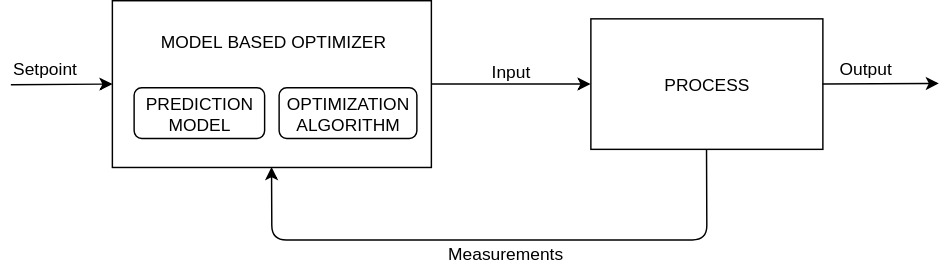
\includegraphics[scale=0.4]{MPC_base_diagram}
	\caption{MPC basic architecture scheme}
	\label{mpc_base_diagram}
\end{figure}
Generally other constraints can be added to the problem in order for example to keep the state variables within feasible ranges. The output of the computation is then the input of the real process to be controlled. In  practice the solution of the problem usually has two main limitations:

\begin{itemize}
\item Model of the process: the nature of the MPC is based on the possibility to forecast the future output of the system by means of a model. Because of that, to have a reliable prediction, we need the system model to be accurate.

\item Optimization algorithm: as mentioned before, the more the system is complex and constraints are added to the problem, the more the problem will be computationally heavy. A proper optimization algorithm needs to be chosen in accordance with the application of the controller.
  
\end{itemize}
Referring to Figure \ref{mpc_horizon_base_scheme}, any controller belonging to MPC family is usually amenable to the following methodology:
\begin{figure}[h!]
	\centering
	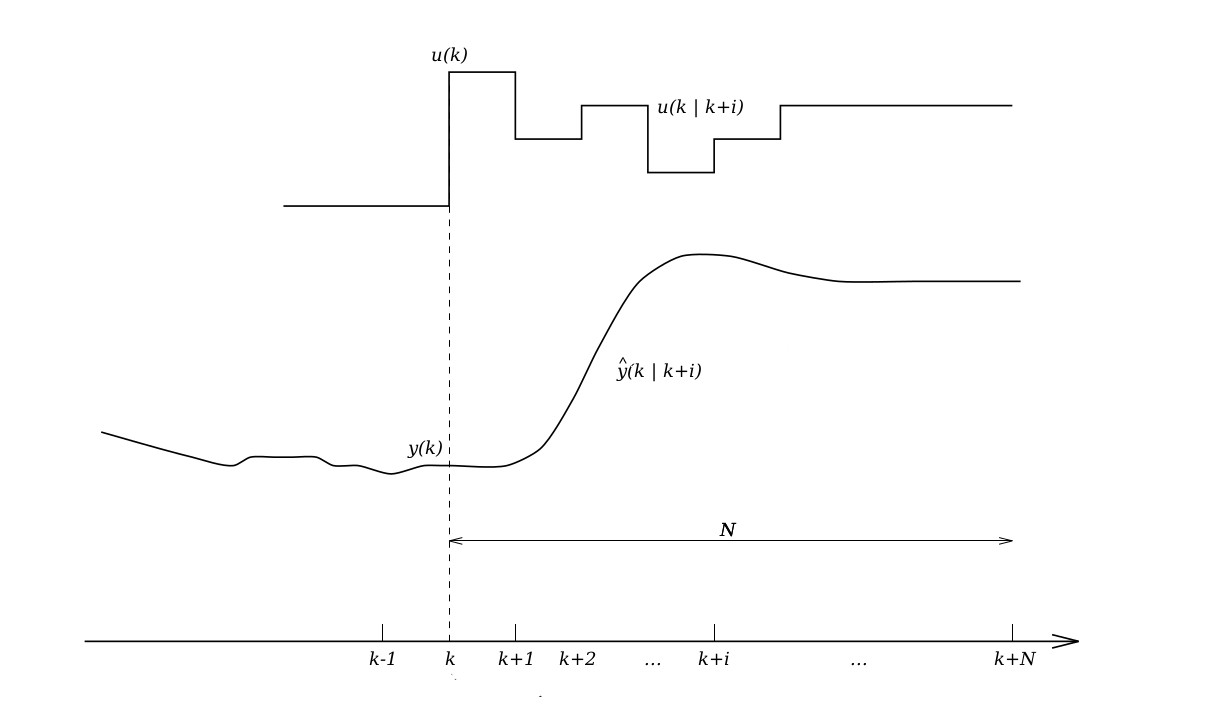
\includegraphics[scale=0.32]{mpc_horizon_base_scheme}
	\caption{MPC strategy}
	\label{mpc_horizon_base_scheme}
\end{figure}

\begin{enumerate}
\item At time instant $k$ future outputs $\hat{y}(k|k+i)$ defined on a prediction horizon $N$ for $i=1,...,N-1$ are predicted starting from past inputs and outputs as a function of the future control actions $u(k|k+i)$, $i=0,...,N-1$.
\item The future control signal is calculated optimizing a given cost function to keep the predicted future output as close as possible to the given reference trajectory $y_d(k+i)$. The objective function is generally defined as a quadratic fuction with respect to this reference trajectory. Control effort term is also usually added to the cost in most cases. If the system is linear and the cost function is quadratic with respect to the error then an explicit solution can be found, otherwise numerical methods have to be used instead.
\item The computed control action $u(k|k)$ is applied to the process then another optimization problem is set based on new measures in order to find $u(k+1|k+1)$ that will be in principle different from $u(k|k+1)$. 
\end{enumerate}
The sequence above repeats continuously at each time step following the so called Receding Horizon principle. In order to be implemented, the model-based optimizer, is designed following the scheme in Figure \ref{scheme_model_based_opt}. 
\begin{figure}[h!]
	\centering
	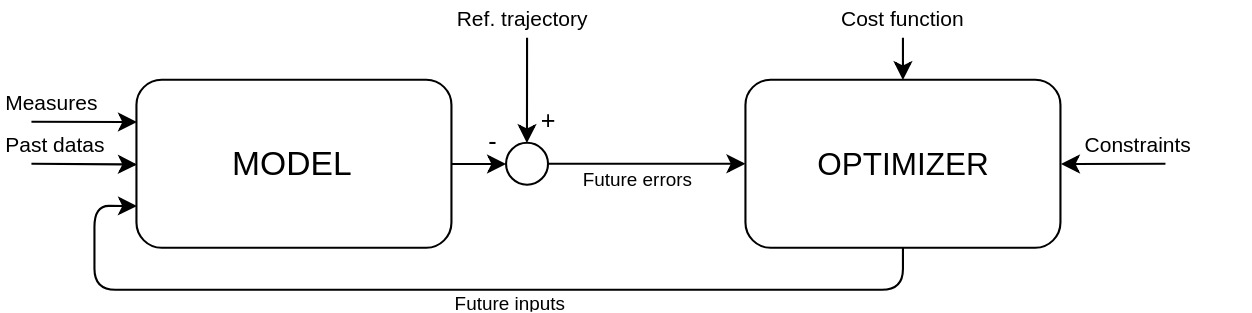
\includegraphics[scale=0.32]{scheme_model_based_opt}
	\caption{Model-based optimizer}
	\label{scheme_model_based_opt}
\end{figure}
The definition of the prediction model can be done in several ways like impulse response, step response, transfer function, state space and more complex representation like neural networks for nonlinear systems. We will refer to the state space representation for the prediction model as it is easy to implement and to integrate.

Let us define the discrete linear time invariant (LTI) model of the process in state space form as:
\begin{equation} \label{system_evolution}
	\begin{split}
		\begin{cases}
			x_{k+1}&=Ax_k+Bu_k \\
			y_{k+1}&=Cx_k
		\end{cases}
	\end{split}
\end{equation}
where $x \in \mathbb{R}^{n_x}$ is the state, $y \in \mathbb{R}^{n_y}$ and $u \in \mathbb{R}^m$ are the output and the control action respectively and $A$, $B$ and $C$ are the matrices of the system. The prediction of the output for this model is given then by:
\begin{equation}\label{system_prediction}
	\hat{y}(k\ |\ k+i)=C\hat{x}(k\ |\ k+i)=C\left[A^i x(k) + \sum_{j=1}^{i} A^{j-1}Bu(k\ |\ k+i-j)\right]
\end{equation}
which can be defined in matrix form as: 
\begin{equation}
\begin{split}
	\left[ \begin{matrix} \hat{y}_{k|1} \\ \hat{y}_{k|2} \\ \vdots \\ \hat{y}_{k|N} \end{matrix} \right] = \underbrace{\left[ \begin{matrix}
	CB		 & 	0	    &	\dots	&	0 		\\
	CAB		 & 	CB	    &	\dots	&	0 		\\
	\vdots	 &  \vdots  &	\ddots	&	\vdots	\\
	CA^{N-1}B & CA^{N-2}B &   \dots   &	CB			
	\end{matrix}\right]}_{\bar{H}}\left[ \begin{matrix} u_{k|0} \\ u_{k|1} \\ \vdots \\ u_{k|N-1} \end{matrix} \right]+ \underbrace{\left[ \begin{matrix} CA \\ CA^2 \\ \vdots \\ CA^N \end{matrix} \right]}_{\bar{T}}x_{k|0}
	\end{split}	
\end{equation}
where for simplicity of notation we refer to $\hat{y}(k\ |\ k+i)$ as $\hat{y}_{k|i}$ and consequently also $x_{k|i}$ and $u_{k|i}$.\\
The definition of the cost function has a strong influence on stability as well as the convergence of numerical optimization methods. A preferrable choice is to consider a positive definite function of the error with respect to the reference trajectory. As the problem can be easily moved a zero-reference problem we will refere to that case. 
\begin{equation} \label{costfunction}
	\begin{split}
		J(x_{k|0},\textbf{u}_k) = \sum_{i=0}^{N-1} \left[\hat{y}_{k|i}^T Q \hat{y}_{k|i} + u_{k|i}^TRu_{k|i} \right] + \hat{y}_{k|N}^T P \hat{y}_{k|N}
	\end{split}	
\end{equation}

where $\textbf{u}_k \in \mathbb{R}^{m\times N}$ with $\textbf{u}_k = [u_{k|0}\ u_{k|1}\ ...\ u_{k|N-1}]^T$ is the control action that has to be found for the predicted horizon. R, Q and P are positive definite weight matrices. Let us write the cost function in matrix form: 
\begin{equation*}
\begin{split}
		J(x_{k|0},\textbf{u}_k)&=x_{k|0}^T Q x_{k|0} + 
		\left[ \begin{matrix} \hat{y}_{k|1} \\ \hat{y}_{k|2} \\ \vdots \\ \hat{y}_{k|N}	\end{matrix} \right]^T \underbrace{\left[ \begin{matrix} 
Q	 		&		 0	  	&  	0	  &  \dots  &  0 \\ 
0 			&  	 Q 	  	& 		0 	  &  \dots  &  0 \\
\vdots  	& 	  \vdots  	&   \ddots   &  \vdots &  0 \\
0 			& 	  \dots  	&      0     &      Q  &  0 \\
0			& 		 0 		&	  \dots   &      0  &  P
\end{matrix} \right]}_{\bar{Q}}
\left[ \begin{matrix} \hat{y}_{k|1} \\ \hat{y}_{k|2} \\ \vdots \\ \hat{y}_{k|N} \end{matrix} \right] +  \\ 
&+\left[ \begin{matrix} u_{k|0} \\ u_{k|1} \\ \vdots \\ u_{k|N-1} 		\end{matrix} \right]^T \underbrace{\left[ \begin{matrix} 
R	 		&		 0	  	&     \dots   &  0 \\ 
0 			&  	     R 	  	&     \dots	  &  0 \\
\vdots  	& 	  \vdots  	&    \ddots   &  \vdots \\
0			& 	  \dots     &        0    &  R
\end{matrix} \right]}_{\bar{R}}
\left[ \begin{matrix} u_{k|0} \\ u_{k|1} \\ \vdots \\ u_{k|N-1}  \end{matrix} \right] 
\end{split}
\end{equation*}

Substituting equation \ref{system_prediction} we obtain:
\begin{equation}
\begin{split} \label{costfunction_expr}
 J(x_{k|0},\textbf{u}_k)&=x_{k|0}^T Q x_{k|0} + (\bar{S}\textbf{u}_k+\bar{T}x_{k|0})^T\bar{Q}(\bar{S}\textbf{u}_k+\bar{T}x_{k|0}) + \textbf{u}_k^T\bar{R}\textbf{u}_k \\ 
 &= \frac{1}{2}\textbf{u}_k^T \underbrace{2(\bar{R}+\bar{S}^T\bar{Q}\bar{S})}_{H}\textbf{u}_k + x_{k|0}^T\underbrace{2\bar{T}^T\bar{Q}\bar{S}}_{F}\textbf{u}_k+\frac{1}{2}x_{k|0}\underbrace{2(Q+\bar{T}^T\bar{Q}\bar{T})}_{Y}x_{k|0} \\
 &=\frac{1}{2}\textbf{u}_k^TH\textbf{u}_k+x_{k|0}F\textbf{u}_k+\frac{1}{2}x_{k|0}Yx_{k|0}
 \end{split}
\end{equation}
Once we have expressed the cost as a function of the measured initial state $x_{k|0}$ and the future control action we can perform the optimization by zeroing the gradient:
\begin{equation}\label{grad_obj_fun}
	\nabla_{\textbf{u}_k}J(x_{k|0},\textbf{u}_k)=H\textbf{u}_k+F^Tx_{k|0}=0
\end{equation}
$\textbf{u}_k$ is then derived inverting \ref{grad_obj_fun}:
\begin{equation}\label{MPC_control_law}
	\textbf{u}_k= \left[
	\begin{matrix}
			u_{k|0} \\ u_{k|1} \\ u_{k|2} \\ \vdots \\ u_{k|N-1}
	\end{matrix}\right] = -H^{-1}F^Tx_{k|0}
\end{equation} 

Consequently the control law can be derivated as:
\begin{equation}
u(t)=-\left[\ I\ 0\ \dots\  0\ \right]H^{-1}Fx(t)\triangleq Kx(t)
\end{equation}
The same result can be obtained from DARE (Discrete-time Algebraic Riccati Equation) as done in \cite{magni2006complementi}.
By means of this result it is possible to implement the MPC with a simple feedback loop. Therefore the derivation of \ref{MPC_control_law} is done offline in this case, the online controller will then be fast, given that the computational effort depend almost only on the inversion of $H$. 
Anyway the assuptions of linear and time invariant system are considerably strong, many of practical systems present nonlinearities and time varying relationship. Because of that, different ways to minimize the cost function in \ref{costfunction} have to be found.
Usually what is done in practice is to use algorithms to perform numerical optimization to find an approximation of the optimal solution. The main issue in the solution of the optimization problem is related to the well-definiteness of the problem choosing properly the cost function formulation. Generally a quadratic form allows to define convex problems in order to guarantee the unicity of the solution.

\subsection{Constraints}

In order to take into account feasibility sets and to guarantee stability, constraints are usually added to the optimization problem that becomes: 
\begin{equation} \label{MPC_problem_constrained}
\begin{split}
		\min_{\textbf{u}_k}\ J(x_{k|0},\textbf{u}_k)&= \sum_{i=0}^{N-1} \left[\hat{y}_{k|i}^T Q \hat{y}_{k|i} + u_{k|i}^TRu_{k|i} \right] + \hat{y}_{k|N}^T P \hat{y}_{k|N} \\
		\textnormal{respecting}\ & 	
		\begin{cases}
			\hat{x}_{k+1}&=A\hat{x}_k+Bu_k \\
			\hat{y}_{k+1}&=C\hat{x}_k
		\end{cases} \\
		\textnormal{s.t.}\qquad
		&\ \ \ \ 0 \leq f(x)\leq 0 \\
		&\ \ \ \ 0 \leq g(u)\leq 0 \\
	\end{split}	
\end{equation}
This notation allows us to introduce both equality and inequality constraints. In practice the constraints are divided into: 
\begin{itemize}
 \item \textbf{Input constraints}: generally represent physical limitation for the control $\textbf{u}_k$ and are defined as "hard" constraints.
 	\item \textbf{State/Output constraints}: usually come from rescrictions into the operational space, they can be both "soft" or "hard".
\end{itemize} 

Hard constraints on the state or on the output gives generally complication in the implementation but soft constraints have to be defined properly according to the application. Moreover "soft" constraints allows a resonable control action to be generated when measured or estimated states moves outside the feasible sets.\\
Given this outline, many are the possible constraints definition: Band Constraints, Overshoot Constraints, Monotonic Behaviour, Nonminimum Phase Behaviour, Actuator Nonlinearities, Terminal State Equality Constraints, Terminal Set Constraints and more, in particular we focus on terminal state equality constraint as it will be useful for the stability proof later on. \\
The terminal state constraint is basically defined as: 
\begin{equation}
\hat{y}_{k|N}=C\left[A^i x_{k|0} + \sum_{j=1}^{i} A^{j-1}Bu_{k|k+N-j}\right]=\bar{y}_N
\end{equation}
that can be rewritten following the form in \ref{MPC_problem_constrained}: 
\begin{equation}
0 \leq \hat{y}_{k|N}-\bar{y}_N \leq 0
\end{equation} 

\subsection{Stability and Feasibility}
In this section stability and feasibility of MPC are investigated in order to give a clear understanding of what done to prove stability of the MPC we developed. To assess feasibility we need to investigate and prove that the problem has a solution; then to prove recursive feasibility, the system should accept a solution $\forall t>0$. As well as feasibility, stability has to be proven in order to have convergence of the performed trajecotry. We will refer to a regulation problem, so the set point will be defined as the origin.
The set $X_{k}$ of initial states $x_{k|0}$ defined for any instant $k$ that ensure feasibility for the MPC problem \ref{MPC_problem_constrained} is defined as:
\begin{equation}
	\begin{split}
		X_{k}=\lbrace\ x_{k|0}\in\mathbb{R}^n\ |\ \exists\  (u_{k|0}, \dots , u_{k|N-1})\ \textnormal{s.t.}\ x_{k|i} \in \mathbb{X}, u_{k|i} \in \mathbb{U},\ &  \\ 
		\forall\  i=0,\dots,N-1,\ x_{k|N} \in \mathbb{X}_f\ \rbrace& \\ 
	\end{split}
\end{equation}
where $\mathbb{U}$ is the region of the control action, $\mathbb{X}_f$ is the region of terminal states and $x_{k|i+1}$ is propagated following the system \ref{system_evolution}. The feasible and unfeasible points in a regulation problem can be visualized on a graph (see \ref{feasibility_image1}) and a region of feasible points can be defined (see \ref{feasibility_region}).

\begin{figure}%
\centering
\subfigure[Feasibility points]{%
\label{feasibility_image1}%
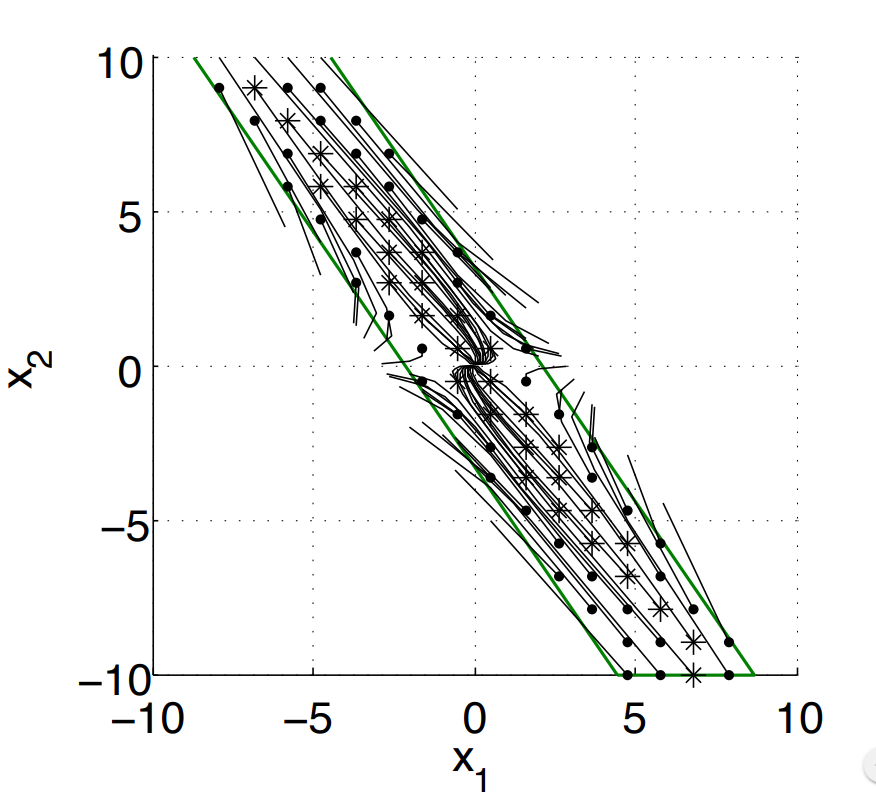
\includegraphics[scale=0.2]{feasibility_image1}}%
\qquad
\subfigure[Feasibility region]{%
\label{feasibility_region}%
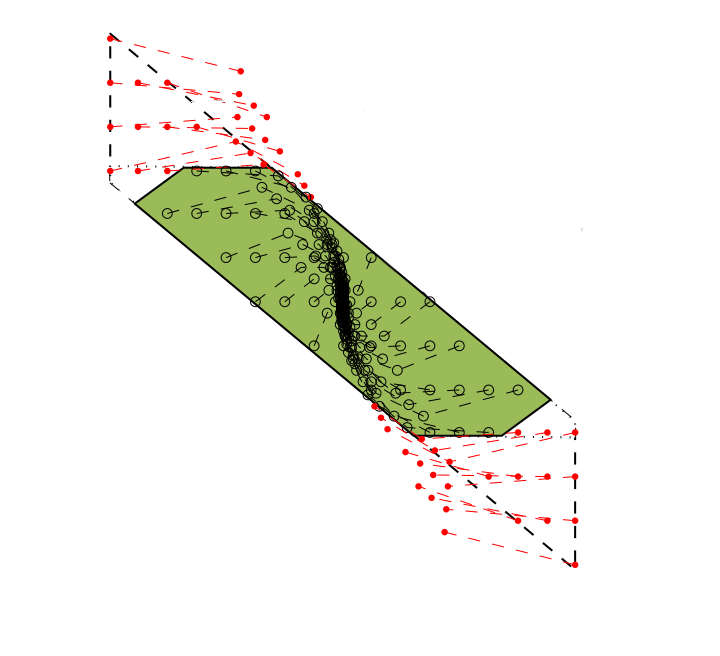
\includegraphics[scale=0.25]{feasibility_region}}%
\caption{Feasibility set}
\end{figure}

Feasibility of a point does not guarantee the feasibility of the following inputs generated by the control action. Because of that Recursive feasibility has to be assessed. That means to show that:
\begin{equation}
\begin{split}
&\ \ \ \ \ \ \ \ \ \forall\ k\ \exists\  \textbf{u}_k\in \mathbb{U}\ \  \textnormal{s.t. } \\ 
\textnormal{given } &x_{k|0} \in \mathbb{X}, \  x_{k|i} \in \mathbb{X}\  \forall i = 1,\  \dots\ , N-1   
\end{split}
\end{equation}
\begin{figure}[h!]
	\centering
	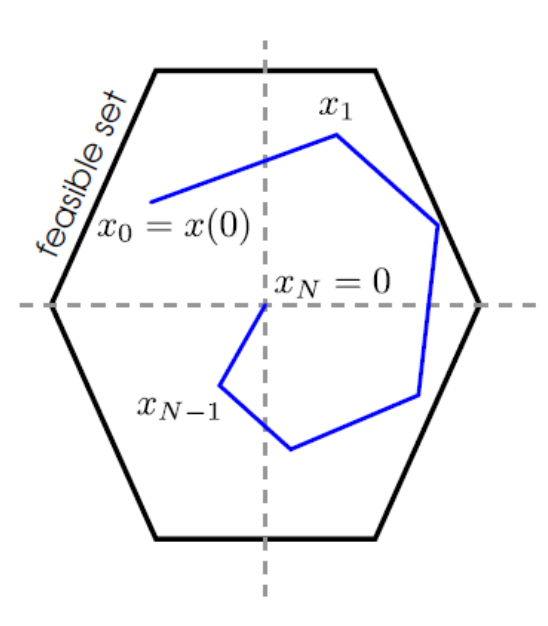
\includegraphics[scale=0.27]{feasible_image2}
	\caption{Recursive feasibility}
	\label{feasible_image2}
\end{figure}

While feasibility proof is straightforward because it is only affected by outputs hard constraints, stability is difficult to assess in some cases.
Stability is a complex function of $N, Q, R, P, \mathbf{u}$ and admissible outputs of the system.
There are many well studied stability proofs for MPC problems:

\begin{itemize}
\item Infinite horizon MPC (N = $\inf$) with no additional constraints
\item Terminal point constraints ($x_{k|N}=0$)
\item Relaxed terminal constraints ($x_{k|N} \in \mathbb{X}_f $)
\end{itemize}

The equilibrium point of a controlled system is said to be Lyapunov stable in $\mathbb{X}$ if $\forall k \in \mathbb{N}$
\begin{equation}
\begin{split}
\forall& \epsilon > 0, \exists \delta(\epsilon) >0 \textnormal{ such that } \forall x_{k|0} \in \mathbb{X}: \\
&||x_{k|0}|| \leq \delta(\epsilon) \implies ||x_{k|i}|| < \epsilon \ \ \forall i \in \mathbb{N}
\end{split}
\end{equation}

Stability proof is generally made by showing that the cost function $J$ to be minimized is a Lyapunov Function and admits an equilibrium point in the origin (regulation problem). If $J$ is a Lyapunov function, the equilibrium point is stable with region of attraction $\mathbb{X}$.

A function $V:X\rightarrow\ \mathbb{R}_+$ is a Lyapunov function if $\forall\ x \in \mathbb{X}$:
\begin{equation} \label{Lyap_func}
\begin{split}
	V(x)>0 \ \ & \forall x \neq 0 \\
	V(0)=&\ 0 \\
	V(x_{k+1})-V(&x_{k}) \leq 0
\end{split}
\end{equation}

In order to guarantee convergence, asymptotic stability in $\mathbb{X}$ of the equilibrium point has also to be verified. Hence it is needed to verify that the equilibrium point is Lyapunov stable and attractive in $\mathbb{X}$ ($\lim_{k \to \infty}||x_k||=0\ \forall\ x \in \mathbb{X}$). 
That can be verified by extending \ref{Lyap_func} asking: 
\begin{equation}
	V(x_{k+1})-V(x_{k}) < 0
\end{equation} 
Now let us consider for simplicity the case in which $C=I$ so the system in \ref{system_evolution} becomes:
\begin{equation*}
x_{k+1}=Ax_k+Bu_k
\end{equation*}

We will assess stability by means of terminal constraints imposition (i.e. $x_{k|N}=0$) considering the quadratic cost function in \ref{costfunction} with  $J(x_{k|0},\textbf{u}_k)=J_k(x_0,\textbf{u})$
\begin{equation}
\begin{split}
J_k(x_0,\textbf{u}) &= \sum_{i=0}^{N-1} \underbrace{\left[x_{k|i}^T Q x_{k|i} + u_{k|i}^TRu_{k|i} \right]}_{q(x_i,u_i)} +\ \underbrace{x_{k|N}^T P x_{k|N}}_{p(x_N)} \\
\textnormal{and}\ \  x_{k|N}&=0
\end{split}
\end{equation}

Recursive feasibility has first to be verified: assuming the feasibility of the point $x_0$ and defining $[u_0^*,\ u_1^*,\ \dots,\ u_{N-1}^*]$ the optimal control sequence computed minimizing $J_0(x_0,\textbf{u})$, following the MPC strategy, the control action applied to the system will be $u_0^*$. The evolution of the system will then be $x_1=Ax_0+Bu_0^*$.
Now at instant $k=1$ the control sequence $[u_0^*,\ u_1^*,\ \dots,\ u_{N-1}^*,\ 0]$ is feasible because applying a null control input and given that $x_N=0$ the resulting final state is $x_{N+1}=0$. This implies that, in presence of end point constraints, the recursive feasibility is verified assuming $x_0$ feasible.

Once feasibility has been assessed, stability has to be investigated by checking if $J$ is a Lyapunov function. So, since we are interested in asymptotic stability, we need to verify:
\begin{equation}
J_0^*(x_1)<J_0^*(x_0)\ \ \ \forall x_0 \neq 0
\end{equation}
Follows that:
\begin{equation}
	\begin{split}
		&J_0^*(x_0)= \underset{=0}{\cancel{p(x_N)}}+\sum_{i=0}^{N-1} q(x_i,u_i^*) \\
		&J_0^*(x_1) \leq \tilde{J}_0(x_1)=\sum_{i=1}^{N}q(x_i,u_i^*) \\
		 = \sum_{i=0}^{N-1}&q(x_i,u_i^*)-q(x_0,u_0^*)+q(x_N,u_N) \\
		 &\ =\  J_0^*(x_0)-q(x_0,u_0^*)+\underset{=0}{\cancel{q(0,0)}} \\
	\end{split}
\end{equation}

Then what can be said is that:
\begin{equation}
	J_0^*(x_1)-J_0^*(x_0)\leq \tilde{J}_0^*(x_1) - J_0^*(x_0) \leq -q(x_0,u_0^*) \leq 0
\end{equation}

Hence, $J^*(x)$ is a Lyapunov function, so the point $x_N=0$ is an asymptotically stable point for the control law. This concept can be generalized for different kind of problems. Anyway, as mentioned before, there are other ways to verify stability which depends on how is the problem defined. Summarizing, terminal constraints imposition provides a sufficient condition for stability.

\subsection{Nonlinear Model Predictive Control (NMPC)}

The basic concepts of MPC have been investigated so far considering linear systems. In general, most of the systems are nonlinear, but even in presence of nonlinearities the use of linear controllers like linear MPC is widely diffuse. There are two main reasons for that: on one hand approximating the model of the system as linear gives good results when it moves in the neighberhood of a stationary point, on the other hand the system parameter estimation for linear systems based on measurements is relatively easy. Futhermore, the minimization of a quadratic cost function in presence of a linear system (i.e. quadratic programming) has been well studied and many commercial products are available (see table \ref{mpc_usage_table}). Moreover, in fast sampling time applications the usage of a linear model provides faster solving time in order to keep the time used to solve the optimization problem lower than the sampling time of the system.
Nevertheless there are cases for which the dynamic response of the resulting linear controller is unacceptable, expecially in highly nonlinear systems or in applications where the dynamic parameters of the system may change over time. In those cases the adoption of nonlinear models is required. 
There is nothing in the theory overviewed in the previous section that prevent the usage of a nonlinear system, therefore the extension of what has been done to nonlinear models is straightforward, at least conceptually. Since state space models are the most used and can be easily extended to consider nonlinearities, instead of the system expressed in \ref{system_evolution}, we will consider:
\begin{equation}
\begin{split}
\begin{cases}
x_{k+1}&=f(x_k,u_k) \\
y_{k+1}&=g(x_k)
\end{cases}
\end{split}
\end{equation} 
Now, given that $x_k$ is the state vector we can see that this representation allows us to represent both single-variable and multi-variable systems. If we consinder as an example the nonlinear system:
\begin{equation}
y_{k+1}=0.9y_k+u_k^{\frac{1}{4}}
\end{equation}
figure \ref{linearvsnl} compares the response of the system when controlled with linear MPC approximating it with $y_{k+1} = 0.9y_k+u_k$ (in black) and when it is controlled with NMPC (in grey). We can see the response of the linear model-based controller oscillates for the first set point values while the nonlinear model-based is quite good. 
\begin{figure}[h!]
	\centering
	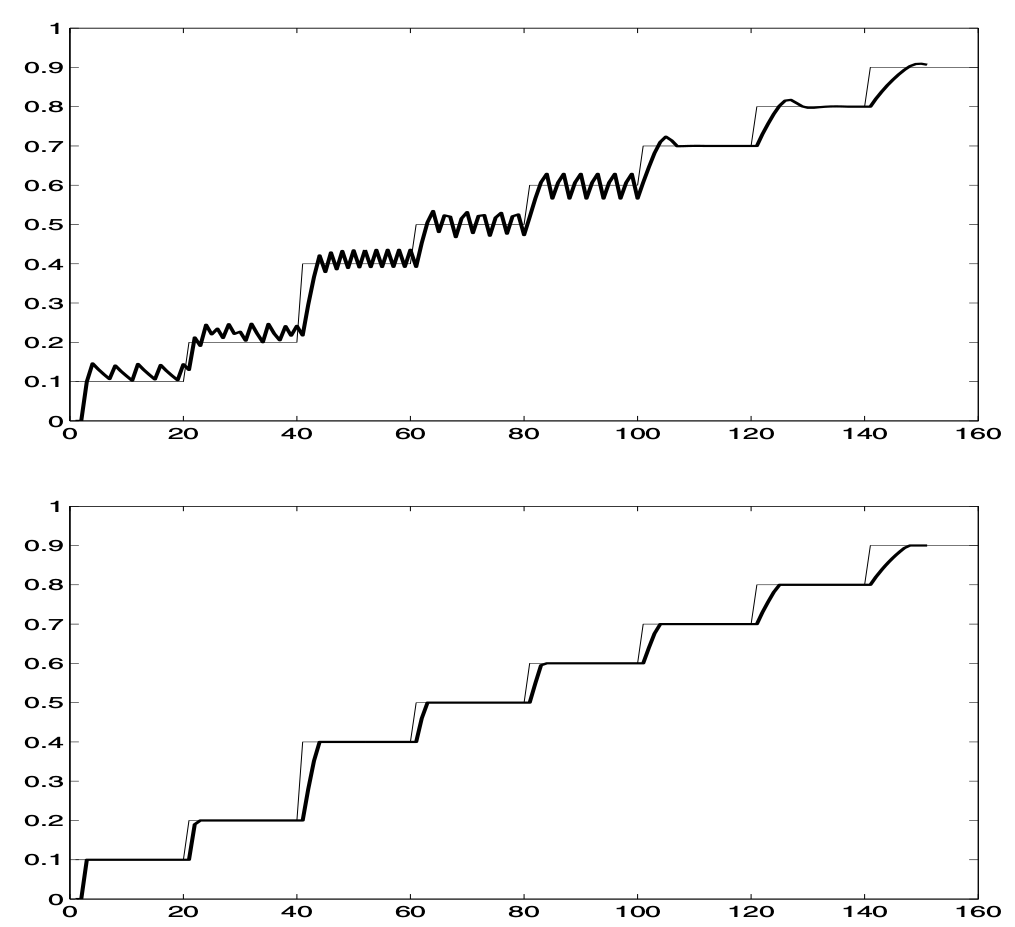
\includegraphics[scale=0.25]{linearvsnl}
	\caption{Linear vs. Nonlinear MPC}
	\label{linearvsnl}
\end{figure}\\
However there are many problems that arise from the use of nonlinear systems:
\begin{itemize}
\item The optimization problem becomes non-convex and because of that, finding a solution becomes not trivial. Local minima may occur influencing performances and stability.
\item The study of stability and robustness becomes more complex and it is still an open field in research.
\item The computational time becomes a variable that has to be taken into account expecially for high speed systems.
\item The identification techniques in presence of nonlinear models are still an open field and model representation through balance of forces is not always feasible. New thecniques like Neural Networks or deep learning are being studied.
\end{itemize} 
%Even if model parameters identification is an open issue for nonlinear systems, this is not the only difficulty related to nonlinear MPC. The increase of computational time required and reliability of the solution have to be taken into account when dealing with online applications of NMPC. 
Nonlinear problems (NLP) are usually solved using Sequential Quadratic Programming (SQP) techniques which are an extension of Newton-type methods for converging the solution of the KKT conditions of the given problem (see \cite{skkt}). The main challange in solving the problem is to guarantee convergence even in presence of ill conditioning and extreme nonlinearities.
In general if the time given to solve the NLP is not sufficient at one step, the last iteration $u_k$, which satisfies the local linear approximation to the constraints, is sent to the system, although it may violate the original constraints. Many approaches have been developed in the years to overcome the difficulties in solving online a NLP dealing with suboptimal solutions and fast convergence. 
\\\\Since now we reviewd basic concepts of MPC logic in order to give an overview of what MPC is based on. Note that what showed can be easily extended for LTV systems since the time dependence of the parameters doesn't affect the cost function definition neither the stability proof.